\section{Graph construction}
\label{sec:ftp_graph}

In the previous section, it was shown that the proposed Flying Tourist Problem and the classical Traveling Salesman are closely relate, but differ in some key aspects. One of these aspects is the time-dependency to which every arc of the FTP is subject to, and to which the TSP is not. 

One of the major consequences of the time-dependency of the FTP is that it requires a three dimensional weight matrix to describe the arcs, where $c_{ij}^t$ correspond to the weight of the arc which goes from node $i$ to node $j$ at time $t$. It should also be noted that this weight matrix is not symmetric, that is, in general, $c_{ij}^t \neq c_{ji}^t$.

While a Traveling Salesman Problem instance is usually described by an $n*n$ weight matrix, the FTP requires an $((n+2)*(n+2))*t$, where the additional two nodes arise from the initial and final nodes, which are not part of the set of nodes to visit. Moreover, the $(n+2)*(n+2)$ bi dimensional weight matrix spans over a third dimensions, representing time. Thus, if the trip spans over $t$ time units, than there are $t$ 

While the Traveling Salesman has a weight matrix of $n*n$ entries, the Flying Tourist Problem requires a weight matrix with $((n+2)*(n+2))*t$ entries (however, note that not all of these entries are necessary).
This is, if the trip span over $t$ time-units, than for each of these time-units, there is a bi dimensional weight matrix describing the weight of each arc connecting any two nodes at that given time.

Despite the FTP weight matrix being three dimensional, it is possible to visualize the problem in two dimensions. Recall the FTP example considered in section \ref{sec:ftp}, together with the multipartite graph illustrating it.
This example spans over 7 time-units, and for each of these time-units, there are $3*3$ arcs connecting the 3 nodes to visit. Note that we have disregarded the arcs connecting these 3 nodes to the depot, since they are not relevant.
Furthermore, the arcs connecting the same node, which simply correspond to a time transition, have a null weight.

TO BE CONTINUED


While the TSP is completely described by an $(n*n)$ weight matrix, the FTP requires an $((n+2)*(n+2))*t$ three dimensional matrix. That is, the trip might span over a period of $k$ time-units, and for each of these time-units, there is an (n+2)*(n+2) weight matrix for the arcs of the problem. Note that the two "extra" nodes, relative to the TSP, arise from the additional initial and final nodes.





That is, the Traveling Salesman can be described by a two dimensional cost matrix, of dimensions $n*n$, where each entry of the cost matrix corresponds to a given weight of an arc connecting two nodes. In its turn, the weight of an arc connecting two nodes in a FTP instance depends on the period of time 



%% ----- use this figure to explain the arc families -----
\begin{figure}[htpb]
  \centering
  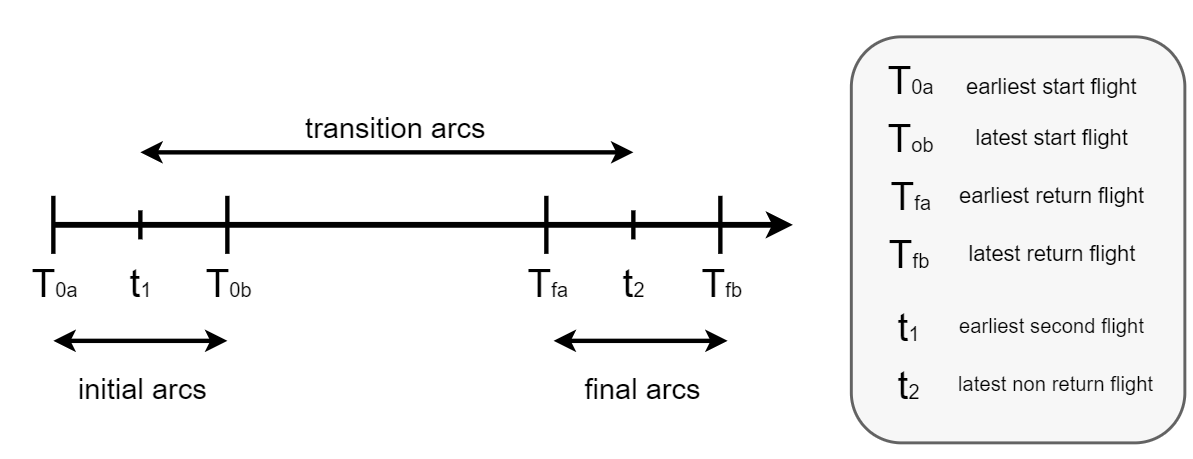
\includegraphics[width=\textwidth]{./Figures/system_design/flights_times.png}
  \caption{Illustration of the distribution in time of the initial, final and transition arcs.}
  \label{fig:multipartite_times} 
\end{figure}





















----------------- old -----------------

\todo{Simplify things. Remove the excess and vaguenes. Try something like this. Define a start node. 2) Schedule a date. 3) Decide where to fly to. 4) Get the possible flights. 5) Decide which are best.}
By considering the presented FTP definition, the total number of layers ($k$) of
the devised multipartite graph represents the total time span between the
earliest date at which the trip might start and the latest date in which it
should finish. The arcs that connect those nodes are divided into three groups:
\textit{initial}, \textit{transition} and \textit{final} arcs.

The \textit{initial} arcs are those which might initiate the trip. Consequently,
they must start at node $v_0$, at a time $t \in T_0 = [T_{0m}, T_{0M}]$,
connecting $v_0$ to every node in $V$. There are a total of $k_i = T_{0M} -
T_{0m} + 1$ layers for the initial arcs.

Conversely, the \textit{final} arcs are those that connect every node in $V$ to
the return node, $v_{n+1}$. There are as many final layers as there are initial
layers, and the final layer extends from $T_{fm}$ to $T_{fM}$, where $T_{fm}$ =
$T_{0m} + \sum(D)$ and $T_{fM}$ = $T_{0M} + \sum(D)$, where $\sum(D)$
corresponds to the summation of all entries belonging to $D$. In the example
depicted in Figure~\ref{fig:multipartite_sol}, there is a single initial and
final layer, since there is only one possible start date.

The \textit{transition} arcs are those which fully connect the $N$ nodes
belonging to $V$. The earliest transition arc occurs at a time no sooner than
$t_1 = T_{0m} + min(D)$, where $min(D)$ corresponds to the lowest entry of the
set of staying durations. Hence, if the trip starts by transiting an initial arc
at time $T_{0m}$, the first transition arc might only be traversed $min(D)$
time-units later. By following a similar approach, the latest transition arc can
occur no latter than $t_2 = T_{0M} + \sum(D) - min(D)$. Thus, there are a total
of $k_2 = t_2-t_1+1$ transition layers, and $k_2*n*(n-1)$ transition arcs.

The union of the initial, transition and final arcs gives the set $A$ of all the
arcs, which may be used to construct a solution to the requested trip. 

Having the information relative to the multipartite graph associated to the
devised FTP, it is now possible to construct a three-dimensional array matrix
representing this problem, where each entry of the array corresponds to an arc
connecting two nodes, at a particular moment in time. This weight matrix is
initialized with a very high cost value (as to reject arcs which may not be part
of the solution), and every entry of it is updated according to the information
of the multipartite graph and the respective objective function. Finally, this
weight matrix may be used as input for the optimization system (see
section
\todo{Insert reference}).
%~\ref{sec:optimization}).

Although it is clear that any arc $a \in A$ corresponds to a particular flight,
it should be noted that no specific or limiting assumption was considered up
until now. Instead, it was assumed an entirely abstract arc definition,
connecting two nodes at a specific moment in time. In order to transform this
set of arcs into a corresponding set of flights, it is necessary to obtain
real-world flight data from some external source. This will be further detailed
in section
\todo{Insert reference}
%~\ref{sec:system}.







